\documentclass[a4paper]{jpconf}
\usepackage[utf8]{inputenc}
\usepackage{graphicx}
\usepackage{lmodern}
\bibliographystyle{iopart-num}


\begin{document}
\title{The Neutron Monitor Control Panel}

\author{O. García-Población$^{1,2}$, H. Ivanov$^2$, I. García-Tejedor$^{1,2}$,
J. J. Blanco$^{1,2}$, J. Medina$^{1,2}$, R. Gómez-Herrero$^{1,2}$, E.
Catalán$^{1,2}$ and D. Radchenko$^{2}$}

\address{$^1$ Space Research Group, University of Alcalá, Spain}
\address{$^2$ Castilla-La Mancha Neutron Monitor, Parque Tecnológico de Guadalajara, Spain}

\ead{oscar.gpoblacion@uah.es}

\begin{abstract}
    This work presents the current status and future plans of NMCP, a new
    software developed to aid the operator in typical station maintenance and
    configuration operations. This software is integrated with new the NOAS
    data acquisition system and can be accessed using a supported web browser.
    If features a visual inspection tool to help the operator to identify
    spikes in the data, trace the origin of the spike back to the raw readings
    of each counter tube and pressure reading, and mark the data as invalid in
    the Neutron Monitor Database if desired. The software also provide
    information about station operation status, some descriptive statistics
    about current data being recorded and, in the future, will provide an
    interface to configure station parameters.
\end{abstract}

\section{Introduction}

%% Aquí hay que hablar de:
%% NMDB data quality. The origin of the spikes. The revision mechanism at NMDB.
%% The need of controlling monitor operation and data. The data acquisition system and
%% how it is related with the operation of the station and its data quality.
Neutron Monitor data is widely used by researchers in different research fields not necessarily related with cosmic rays. That's why the NMBD
puts effort into delivering data with the best quality possible. The data is also used in real time GLE alarm systems and other real time
applications therefore the data quality protocol must be applied in real time. Eventually the data will be revised by a human supervisor to 
ensure the correct behaviour of the quality protocol. By quality protocol we refer to all the methods and techniques used such as:
\begin{itemize}
	\item   Detection of abnormal data, commonly referred as spikes.
	\item   Detection of inactivity which will lead to a notification to the team responsible for the neutron monitor station.
	\item   Monitor neutrons are usually formed by 18 counter tubes. A malfunction in a single tube won't affect the overall value measured
	  	by the neutron monitor but it's not something desirable. This leads us to the need of monitoring and detection of malfunctions
		separately in each of the tubes.  
	\item	Detection of changes regard of the historical activity. Instrumental changes or changes in the immediate environment can cause 
	  	overall changes in the measured values of a monitor neutron. Detecting and correcting those changes is desirable.
	\item 	Comparing the data from one NM station with the data of different nearby NM stations. Detecting isolated events in one NM
	  	station indicates us that there is a malfunction in that NM station.	
\end{itemize}
Once detected the corrupt data, most of the times it can be traced down to its cause. Most of the times those malfunctions are caused by the
instruments forming the data acquisition system. Detecting the corrupt data and its cause helps us to improve and learn more about the data
acquisition system. In order to make easier the detection of the corrupt data we are working in the development of a Web tool which will help
us detect the corrupted data. The Web application makes use of dynamically generated plots which aim to highlight possible corrupted data.


blabla \cite{Garcia2014}
blabla \cite{Medina2013}
blabla \cite{NMDB2011}
blabla \cite{Forbush1938}

\section{System architecture}

%% ¿Qué partes constituyen el nuevo software? ¿Cómo se integran esas partes
%% entre sí y con el sistema de acquisicion de datos? Es la parte del poster que
%% habla de ``Architecture''

	Blah blah blah
	On figure \ref{fig:arch} we can see blah

	\begin{figure}[h]
		\centering
		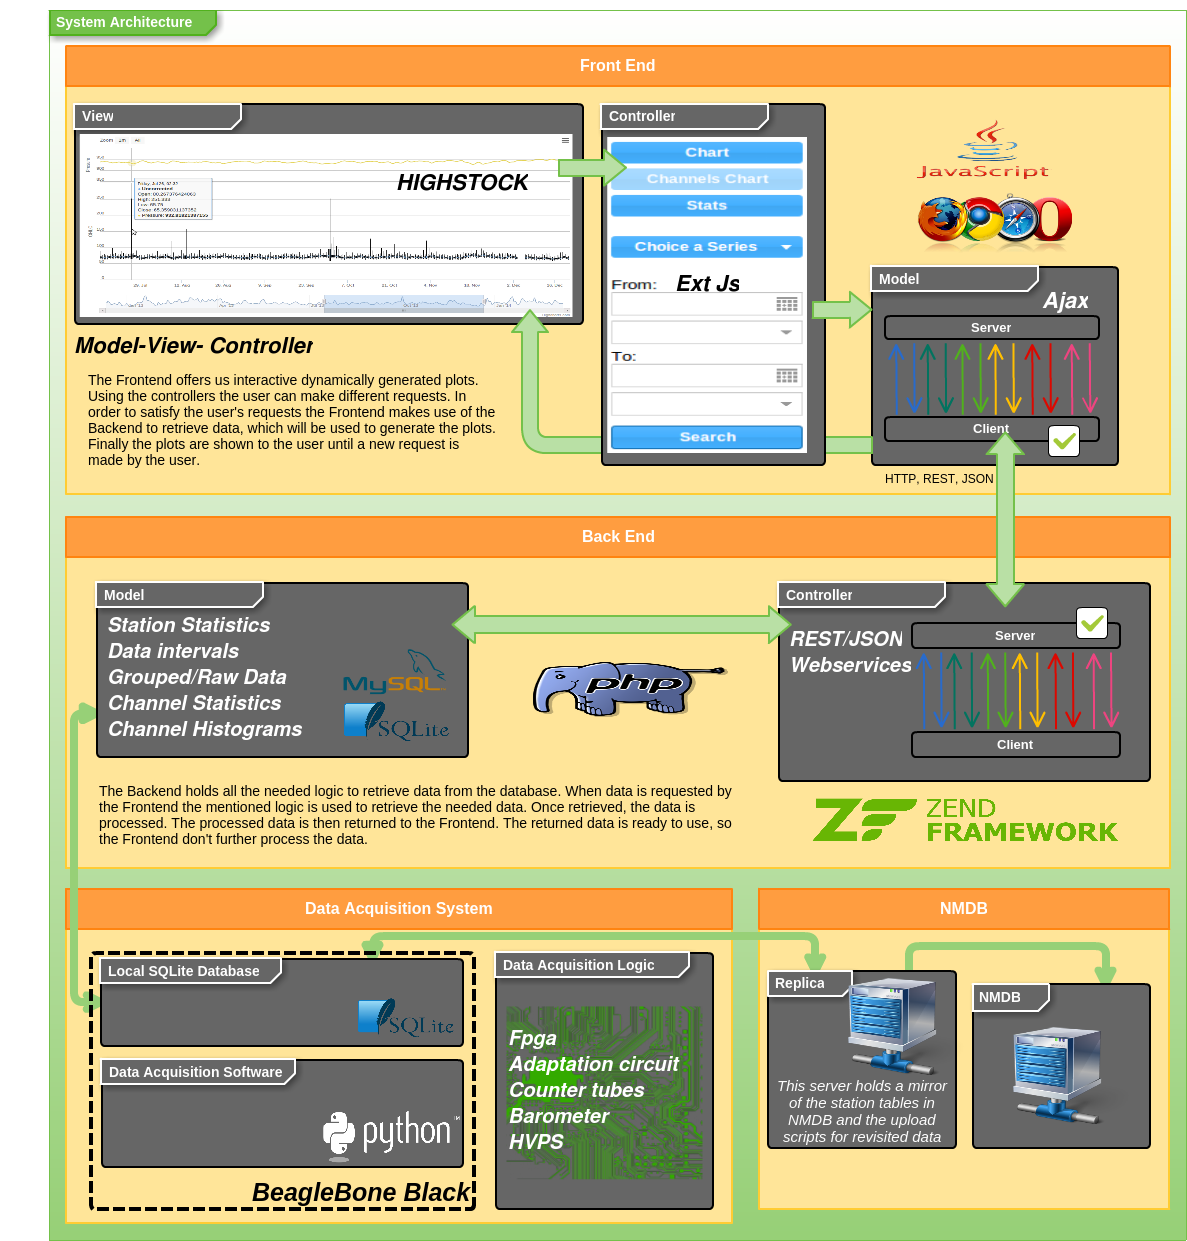
\includegraphics[keepaspectratio, width=1\textwidth]{./resources/Architecture.png}
		\caption{Architecture}
		\label{fig:arch}
	\end{figure}

\section{The spike tool}

%% Aquí hablaremos concretamente del spike tool. Sobre todo de cómo funciona
%% cara al usuario.

\section{Future work}

The neutron monitor control panel is a natural evolution of the new data
acquisition system designed for neutron monitors and it is under active
development to add new useful features in the near future. Some of these future
features are summarized bellow.

\begin{description}
    \item[Online statistics] The control panel will include a module for
        descriptive statistics that will be calculated in real time from the
        counter tubes raw readings. This will help to identify drifts in the
        behavior of the detectors and to apply the appropriate actions to
        maintain data quality.
    \item[Station reconfiguration] This will allow the operator to disconnect a
        counter from the station without affecting global station count. This
        can be useful to carry on maintenance operations such as counter tube
        diagnostics. 
    \item[Station parameter setup] New electronics allow the remote control of
        some parameters, for example the high voltage power supply set point,
        the remote database for data upload, backup policies, etc.
    \item[Alarms and push notifications] When connectivity allows it, it will
        be possible to configure alarms and notification to recipients using
        the new push mobile technologies, for example if the station is no
        longer uploading data to NMDB or if data is out of quality standards
    \item[Detector response histogram] A new design from the New
        Hampshire University of the front-end amplifiers provides a pulse which
        width is proportional to the energy of the incident particle. The new
        FPGA IP-core running in the NOAS, the second version of our data
        acquisition system, is able to read these pulses and to generate an
        histogram with the distribution of the pulses energy over a given time
        interval. This will enable a mechanism for non-intrusive diagnostics of
        the counter tubes. 
\end{description}


\subsection*{Acknowledgments} 
The authors would like to thank the OMNIweb team and the Neutron
Data Base for the use of their data. This work has been partially supported by
Ministerio de Ciencia y Tecnologia through the project AYA2012-39810-C02-01
Pic du Midi and Kiel.....



\section*{References}
\bibliography{iopart-num} 

\end{document}


